\documentclass[a4paper,12pt]{article}

% --- PACKAGES ---
% =============================
% --- ENCODAGE & TYPOGRAPHIE ---
% =============================
\usepackage[utf8]{inputenc}
\usepackage[T1]{fontenc}
\usepackage{lmodern}
\usepackage{microtype}
\usepackage{setspace}
\usepackage{indentfirst}
\usepackage{ragged2e}
\usepackage{parskip}

% Guillemets francais « » : commandes \og ... \fg sans charger babel
% (babel-french doublerait les espaces des « ~: » deja presents dans le texte)
\providecommand{\og}{\guillemotleft\,}
\providecommand{\fg}{\,\guillemotright}

\usepackage{siunitx}
\sisetup{detect-all, output-decimal-marker={,}}

% =============================
% --- MISE EN PAGE ---
% =============================
\usepackage[margin=2.5cm]{geometry}
\usepackage{fancyhdr}
\usepackage{titlesec}
\usepackage{needspace}

% =============================
% --- COULEURS & GRAPHISME ---
% =============================
\usepackage[table]{xcolor}
\usepackage{transparent}
\usepackage{tikz}
\usetikzlibrary{shadows}

% =============================
% --- IMAGES / PDF / WRAP ---
% =============================
\usepackage{graphicx}
\usepackage{wrapfig}
\usepackage{pdfpages}
\usepackage[absolute,overlay]{textpos}

% =============================
% --- POLICE PAR DÉFAUT ---
% =============================
\usepackage{helvet}
\renewcommand{\familydefault}{\sfdefault}

% =============================
% --- TABLEAUX ET LISTINGS ---
% =============================
\usepackage{tabularx}
\usepackage{array}
\usepackage{booktabs}
\usepackage{listings}
\newcolumntype{C}{>{\centering\arraybackslash}X}
\renewcommand{\arraystretch}{1.4}

% =============================
% --- HYPERREF & URL ---
% =============================
\usepackage{hyperref}
\usepackage{url}
\usepackage{xurl}

% =============================
% --- ALGORITHMES ---
% =============================
\usepackage{algorithm}
\usepackage{algpseudocode}

% =============================
% --- INFORMATIQUE ---
% =============================
\usepackage{minted}
\usemintedstyle{lovelace}

% =============================
% --- MATH ---
% =============================
\usepackage{amsmath}
\usepackage{amssymb}
\usepackage{amsfonts}

% =============================
% --- ANNEXES & CITATIONS ---
% =============================
\usepackage[toc]{appendix}
\usepackage{csquotes}
\usepackage{tcolorbox}

% =============================
% --- PIFONT (CHECKS ICONES) ---
% =============================
\usepackage{pifont}
\newcommand{\good}{\ding{51}}
\newcommand{\bad}{\ding{55}}

% =============================
% --- WARNINGS LaTeX ---
% =============================
\hfuzz=2pt
\hbadness=10000

% =============================
\usepackage[framemethod=tikz]{mdframed}

% --- STYLES ---
% --- STYLES ---

% ========================
%       INDENTATION
% ========================
\setlength{\parindent}{1.5em}      % Indentation automatique des paragraphes

% ========================
%         COULEURS
% ========================
\definecolor{title1}{RGB}{32, 94, 153} % Bleu foncé (titres de sections)
\definecolor{title2}{RGB}{75, 147, 215} % Bleu clair (titres de sous-sections)
\definecolor{footer}{RGB}{75, 147, 215}

% ========================
%   FORMATTAGE DES TITRES
% ========================
\titleformat{\section}
  {\color{title1}\normalfont\Large\bfseries\fontfamily{cmss}}
  {\color{title1}\thesection}{1em}
  {\MakeUppercase}
  [\noindent\color{black}\rule{\textwidth}{0.5pt}]

\titleformat{\subsection}
  {\color{title2}\normalfont\large\bfseries\fontfamily{cmss}}
  {\color{title2}\thesubsection}{1em}
  {\MakeUppercase}
  [\noindent\color{black}\rule{\textwidth}{0.4pt}]

% ========================
%   PERSONNALISATION LISTES
% ========================
\renewcommand{\contentsname}{Table des Matières}
\renewcommand{\listfigurename}{Table des Figures}
\renewcommand{\appendixname}{Annexe}

% ========================
%    STYLE DES PAGES
% ========================
\pagestyle{empty} % Pas d'en-tête ni pied de page par défaut

% ========================
% POSITIONNEMENT TEXTBLOCK
% ========================
\setlength{\TPHorizModule}{1cm}
\setlength{\TPVertModule}{1cm}

% ========================
\hypersetup{
    colorlinks=true,
    linkcolor=black,
    urlcolor=blue,
    citecolor=blue
}

% ========================
%     STYLE DES CAPTIONS
% ========================
\newmdenv[
  topline=false,
  rightline=false,
  bottomline=false,      % Active la ligne du bas
  linewidth=2pt,         % Épaisseur de la barre verticale
  linecolor=black,       % Couleur de la barre verticale
  innerleftmargin=10pt   % Optionnel : espace après le bloc
  innertopmargin=15pt
]{captionbox}


% Configuration de la coloration syntaxique pour JavaScript
\definecolor{codegreen}{rgb}{0,0.6,0}
\definecolor{codegray}{rgb}{0.5,0.5,0.5}
\definecolor{codepurple}{rgb}{0.58,0,0.82}
\definecolor{backcolour}{rgb}{0.95,0.95,0.92}

\lstdefinestyle{jsstyle}{
    backgroundcolor=\color{backcolour},
    commentstyle=\color{codegreen},
    keywordstyle=\color{magenta},
    numberstyle=\tiny\color{codegray},
    stringstyle=\color{codepurple},
    basicstyle=\ttfamily\footnotesize,
    breakatwhitespace=false,
    breaklines=true,
    captionpos=b,
    keepspaces=true,
    numbers=left,
    numbersep=5pt,
    showspaces=false,
    showstringspaces=false,
    showtabs=false,
    tabsize=2,
    language=Java
}

\usepackage{adjustbox}
\usepackage{enumitem}
\usepackage{pdflscape}
\usetikzlibrary{arrows.meta, positioning, calc, shapes.multipart}

% --- RÈGLES DE MISE EN PAGE ---
% Paragraphes, listes et cases de tableau jamais coupés entre deux pages,
% pas de ligne seule en haut ou en bas de page
\interlinepenalty=10000
\clubpenalty=10000
\widowpenalty=10000
\displaywidowpenalty=10000
% Une liste reste attachée à la phrase qui l'introduit et n'est pas coupée
\setlist{beginpenalty=10000}
\makeatletter
\@itempenalty=10000
\makeatother
% Un titre part à la page suivante s'il ne reste pas la place d'un vrai bloc.
% \needspace redéfini sans son \penalty-100, qui faisait préférer une coupure
% avant chaque titre et laissait de grands blancs en bas de page ;
% pas de coupure forcée si la page est déjà pleine (elle se coupera d'elle-même)
\makeatletter
\renewcommand{\needspace}[1]{\par\begingroup\setlength{\dimen@}{#1}%
  \dimen@ii\pagegoal\advance\dimen@ii-\pagetotal
  \ifdim\dimen@>\dimen@ii\ifdim\dimen@ii>\z@\vfil\break\fi\fi\endgroup}
\makeatother
\usepackage{etoolbox}
\pretocmd{\section}{\needspace{14\baselineskip}}{}{}
\pretocmd{\subsection}{\needspace{10\baselineskip}}{}{}
% Plus d'air autour des tableaux et des schémas centrés
\AtBeginEnvironment{center}{\setlength{\topsep}{14pt plus 4pt minus 2pt}}

% --- TABLES DE MODÉLISATION (TikZ) ---
\definecolor{fait}{RGB}{214, 110, 30}
\tikzset{
	tbl/.style={rectangle split, rectangle split parts=2, draw=title1, line width=0.6pt,
		rounded corners=1.5pt, font={\scriptsize\linespread{1.3}\selectfont}, align=left, text width=#1, inner sep=2.5pt,
		rectangle split part fill={title1, white}},
	tbl/.default=2.6cm,
	sous/.style={tbl=#1, draw=title2, rectangle split part fill={title2, white}},
	sous/.default=2.4cm,
	fait/.style={tbl=#1, draw=fait, rectangle split part fill={fait, fait!7}},
	fait/.default=3cm,
	lien/.style={draw=black!55, line width=0.6pt},
}
% \tb{NOM}{attributs} : en-tête + liste des attributs
\newcommand{\tb}[2]{\textcolor{white}{\textbf{#1}}\nodepart{second}#2}
\newcommand{\pk}[1]{\underline{#1}}
\newcommand{\fk}[1]{\##1}
\newcommand{\mes}[1]{\textcolor{fait}{\textit{#1}}}
% Colonnes nom | type du modèle physique
\newenvironment{phys}{\renewcommand{\arraystretch}{1}\begin{tabular}{@{}l@{\hspace{6pt}}>{\color{black!60}\ttfamily}l@{}}}{\end{tabular}}
\newcommand{\legende}{\par\vspace{0.1cm}{\centering\footnotesize
	Légende~: \pk{clé primaire} \quad \fk{clé étrangère} \quad \mes{mesure}\par}}

\begin{document}
\sloppy

% --- PAGE DE GARDE ---
\begin{titlepage}
\thispagestyle{empty}

\begin{center}
    
\includegraphics[height=2cm]{../../../../_Template/assets/img/cesi_logo.png}

    \vspace{0.5cm}
    \rule{12cm}{0.4pt}

    \vspace{0.4cm}
    {\LARGE \textbf{Stockage \& Big Data}}

    \vspace{0.4cm}
    \rule{12cm}{0.4pt}

    \vspace{1cm}
    {\Large \textbf{Workshop | Modélisation multidimensionnelle}} \\[0.3cm]
    \rule{5cm}{0.4pt} \\[0.3cm]
    Mardi 20 octobre 2026
\end{center}

\vfill
\begin{flushleft}
Mazou Marine \\
Fisa Info 25–28 \\
CESI
\end{flushleft}

\end{titlepage}


% --- TABLE DES MATIÈRES ---
\newpage
\tableofcontents

% --- FOOTER ---
% --- FOOTER --- 
\newpage
\pagestyle{fancy}
\setlength{\headheight}{16pt}
\fancyhf{}

\fancyfoot[L]{%
	\transparent{0.5}%
	\textcolor{footer}{\fontsize{16}{18}\selectfont \textbf{\thepage}}%
}

\fancyfoot[R]{%
	\raisebox{-0.7cm}{%
		\transparent{0.5}%
		
\includegraphics[height=1cm]{../../../../_Template/assets/img/cesi_logo.png}%
	}%
}

\renewcommand{\headrulewidth}{0pt}
\renewcommand{\footrulewidth}{0pt}

% --- CONTENT ---
% =====================================================================
%  INTRODUCTION
% =====================================================================
\newpage
\section*{Introduction}
\addcontentsline{toc}{section}{Introduction}

\noindent Les bases de données relationnelles des systèmes \textbf{OLTP} (\textit{Online Transaction Processing}) sont conçues pour enregistrer les opérations du quotidien~: elles sont normalisées et optimisées pour les insertions et les mises à jour. Un \textbf{entrepôt de données} (\textit{data warehouse}) ou un \textbf{magasin de données} (\textit{data mart}) répond à un autre besoin~: analyser l'activité dans le temps à l'aide de systèmes \textbf{OLAP} (\textit{Online Analytical Processing}).

Ce workshop met en pratique la \textbf{modélisation dimensionnelle}~:
\begin{itemize}
	\item une \textbf{table de faits} contient les \textbf{mesures} numériques à analyser (quantités, montants\dots) et les clés étrangères vers les dimensions. Son \textbf{grain} est le niveau de détail d'une ligne~;
	\item une \textbf{table de dimension} contient les \textbf{axes d'analyse} (qui, quoi, où, quand\dots) et leurs attributs descriptifs, souvent organisés en \textbf{hiérarchies} (jour $\rightarrow$ mois $\rightarrow$ année)~;
	\item le modèle peut être en \textbf{étoile} (dimensions dénormalisées), en \textbf{flocon} (hiérarchies normalisées en sous-tables) ou en \textbf{constellation} (plusieurs tables de faits partageant des dimensions).
\end{itemize}

\noindent Les schémas suivent la même légende~:
\legende

% =====================================================================
%  EXERCICE 1
% =====================================================================
\newpage
\section*{Exercice 1~: du MCD au MLD}
\addcontentsline{toc}{section}{Exercice 1~: du MCD au MLD}

\noindent Le passage du modèle conceptuel (entité-association) au modèle logique relationnel repose sur trois règles~:
\begin{enumerate}
	\item chaque \textbf{entité} devient une \textbf{table}~; son identifiant devient la \textbf{clé primaire}~;
	\item une association \textbf{binaire de type 1-n} (cardinalité maximale 1 d'un côté) disparaît~: la table du côté \og 1 \fg{} reçoit une \textbf{clé étrangère} vers l'autre table. Si la cardinalité minimale est 0, la clé étrangère peut être \texttt{NULL}~;
	\item une association \textbf{n-n} devient une \textbf{table d'association}. Sa clé primaire est composée des clés étrangères des entités reliées, et elle reçoit les attributs portés par l'association.
\end{enumerate}

% ---------------------------------------------------------------------
\newpage
\subsection*{Modèle 1~: association 1-n}
\phantomsection
\addcontentsline{toc}{subsection}{Modèle 1~: association 1-n}

\noindent Une personne réside à \textbf{0 ou 1} adresse, une adresse accueille \textbf{0 à n} personnes. La cardinalité maximale est 1 du côté \texttt{Personne}~: l'association \texttt{Réside} disparaît et \texttt{Personne} reçoit l'identifiant de l'adresse en clé étrangère.

\begin{tcolorbox}[colback=white, colframe=title1, title=MLD -- Modèle 1]
\textbf{PERSONNE} (\pk{ID\_personne}, Nom, Prénom, \fk{ID\_adresse}) \\
\textbf{ADRESSE} (\pk{ID\_adresse}, Voie, CP, Ville)
\end{tcolorbox}

\vspace{0.5cm}
\begin{center}
\begin{adjustbox}{width=0.75\linewidth}
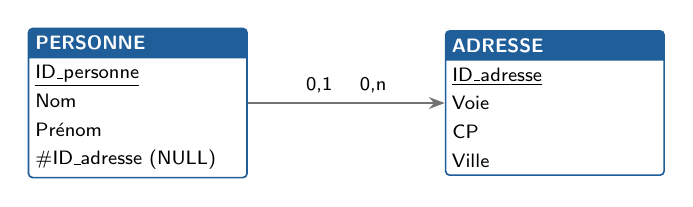
\begin{tikzpicture}
	\node[tbl] (P) {\tb{PERSONNE}{\pk{ID\_personne}\\ Nom\\ Prénom\\ \fk{ID\_adresse} (NULL)}};
	\node[tbl, right=2.5cm of P] (A) {\tb{ADRESSE}{\pk{ID\_adresse}\\ Voie\\ CP\\ Ville}};
	\draw[lien, -{Stealth}] (P) -- node[above, font=\scriptsize]{0,1 \quad 0,n} (A);
\end{tikzpicture}
\end{adjustbox}
\legende
\end{center}

\vspace{0.5cm}
\noindent \texttt{ID\_adresse} est \textbf{nullable} (cardinalité minimale 0)~: une personne peut ne pas avoir d'adresse connue.

% ---------------------------------------------------------------------
\newpage
\subsection*{Modèle 2~: association n-n porteuse d'un attribut}
\phantomsection
\addcontentsline{toc}{subsection}{Modèle 2~: association n-n porteuse d'un attribut}

\noindent Une personne peut résider à plusieurs adresses (dans le temps) et une adresse peut accueillir plusieurs personnes. L'association \texttt{Réside} est \textbf{n-n}~: elle devient une table dont la clé primaire est le couple des deux identifiants. Elle porte la date d'emménagement.

\begin{tcolorbox}[colback=white, colframe=title1, title=MLD -- Modèle 2]
\textbf{PERSONNE} (\pk{ID\_personne}, Nom, Prénom) \\
\textbf{ADRESSE} (\pk{ID\_adresse}, Voie, CP, Ville) \\
\textbf{RESIDE} (\pk{\fk{ID\_personne}, \fk{ID\_adresse}}, Date\_emmen)
\end{tcolorbox}

\vspace{0.5cm}
\begin{center}
\begin{adjustbox}{width=0.9\linewidth}
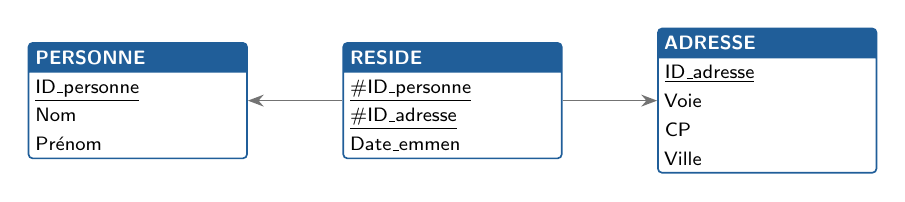
\begin{tikzpicture}
	\node[tbl] (P) {\tb{PERSONNE}{\pk{ID\_personne}\\ Nom\\ Prénom}};
	\node[tbl, right=1.2cm of P] (R) {\tb{RESIDE}{\pk{\fk{ID\_personne}}\\ \pk{\fk{ID\_adresse}}\\ Date\_emmen}};
	\node[tbl, right=1.2cm of R] (A) {\tb{ADRESSE}{\pk{ID\_adresse}\\ Voie\\ CP\\ Ville}};
	\draw[lien, -{Stealth}] (R) -- (P);
	\draw[lien, -{Stealth}] (R) -- (A);
\end{tikzpicture}
\end{adjustbox}
\legende
\end{center}

\vspace{0.5cm}
\noindent Avec cette clé, une personne ne peut être liée qu'\textbf{une seule fois} à une même adresse~: un retour à une ancienne adresse écraserait la date d'emménagement. Le modèle 3 corrige ce point.

% ---------------------------------------------------------------------
\newpage
\subsection*{Modèle 3~: association n-n historisée}
\phantomsection
\addcontentsline{toc}{subsection}{Modèle 3~: association n-n historisée}

\noindent Même règle que le modèle 2, mais l'association porte une \textbf{période} (\texttt{Date\_debut}, \texttt{Date\_fin}). Pour garder tout l'historique, y compris plusieurs séjours d'une même personne à une même adresse, \texttt{Date\_debut} entre dans la clé primaire.

\begin{tcolorbox}[colback=white, colframe=title1, title=MLD -- Modèle 3]
\textbf{PERSONNE} (\pk{ID\_personne}, Nom, Prénom) \\
\textbf{ADRESSE} (\pk{ID\_adresse}, Voie, CP, Ville) \\
\textbf{RESIDE} (\pk{\fk{ID\_personne}, \fk{ID\_adresse}, Date\_debut}, Date\_fin)
\end{tcolorbox}

\vspace{0.5cm}
\begin{center}
\begin{adjustbox}{width=0.9\linewidth}
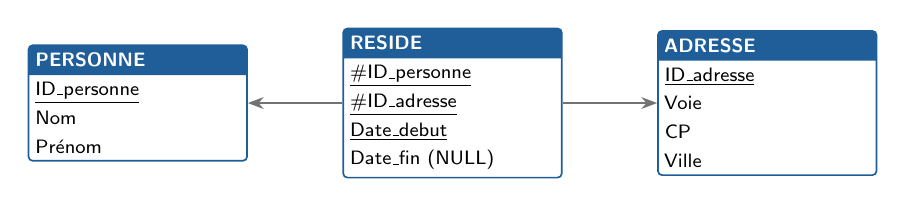
\begin{tikzpicture}
	\node[tbl] (P) {\tb{PERSONNE}{\pk{ID\_personne}\\ Nom\\ Prénom}};
	\node[tbl, right=1.2cm of P] (R) {\tb{RESIDE}{\pk{\fk{ID\_personne}}\\ \pk{\fk{ID\_adresse}}\\ \pk{Date\_debut}\\ Date\_fin (NULL)}};
	\node[tbl, right=1.2cm of R] (A) {\tb{ADRESSE}{\pk{ID\_adresse}\\ Voie\\ CP\\ Ville}};
	\draw[lien, -{Stealth}] (R) -- (P);
	\draw[lien, -{Stealth}] (R) -- (A);
\end{tikzpicture}
\end{adjustbox}
\legende
\end{center}

\vspace{0.5cm}
\noindent Contraintes à ajouter~: \texttt{Date\_fin} vaut \texttt{NULL} pour la résidence actuelle, et \texttt{Date\_fin} $\geq$ \texttt{Date\_debut}. C'est le principe des \textbf{dimensions à évolution lente} (\textit{SCD de type 2}) utilisées dans les entrepôts pour historiser un attribut.

% =====================================================================
%  EXERCICE 2
% =====================================================================
\newpage
\section*{Exercice 2~: ventes d'une entreprise industrielle}
\addcontentsline{toc}{section}{Exercice 2~: ventes d'une entreprise industrielle}

\noindent \textbf{Besoin~:} analyser dans le temps les \textbf{quantités vendues} et les \textbf{coûts associés}, par produit, client, magasin et promotion.

\begin{itemize}
	\item \textbf{Fait~:} la vente.
	\item \textbf{Grain~:} une ligne = un produit vendu à un client, dans un magasin, un jour donné, sous une promotion donnée.
	\item \textbf{Mesures~:} \texttt{quantite\_vendue}, \texttt{cout\_total} (coût associé à la vente) et \texttt{montant\_vente}. Elles sont \textbf{additives}~: on peut les sommer sur tous les axes.
	\item \textbf{Dimensions~:} Temps, Produit, Client, Magasin, Promotion. Les données fournies contiennent aussi \texttt{nom\_employé} et \texttt{mail\_employé}~: les employés enregistrent les clients, on ajoute donc une dimension Employé (performance des vendeurs).
\end{itemize}

% ---------------------------------------------------------------------
\newpage
\subsection*{1. Modèle en étoile}
\phantomsection
\addcontentsline{toc}{subsection}{1. Modèle en étoile}

\noindent Chaque dimension est \textbf{une seule table dénormalisée}~: les hiérarchies (groupe de produit, région, pays\dots) sont des colonnes de la dimension.

\vspace{0.5cm}
\begin{center}
\begin{adjustbox}{width=\linewidth}
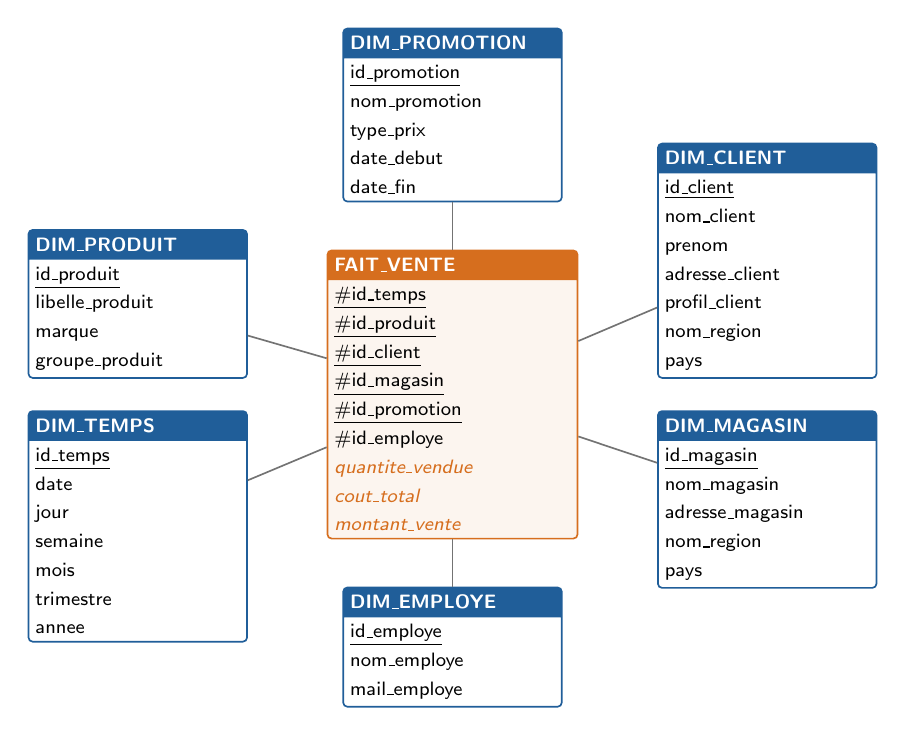
\begin{tikzpicture}
	\node[fait] (F) {\tb{FAIT\_VENTE}{\pk{\fk{id\_temps}}\\ \pk{\fk{id\_produit}}\\ \pk{\fk{id\_client}}\\ \pk{\fk{id\_magasin}}\\ \pk{\fk{id\_promotion}}\\ \fk{id\_employe}\\ \mes{quantite\_vendue}\\ \mes{cout\_total}\\ \mes{montant\_vente}}};

	\node[tbl, anchor=south east] (P) at ($(F.west)+(-1,0.2)$) {\tb{DIM\_PRODUIT}{\pk{id\_produit}\\ libelle\_produit\\ marque\\ groupe\_produit}};
	\node[tbl, anchor=north east] (T) at ($(F.west)+(-1,-0.2)$) {\tb{DIM\_TEMPS}{\pk{id\_temps}\\ date\\ jour\\ semaine\\ mois\\ trimestre\\ annee}};
	\node[tbl, anchor=south west] (C) at ($(F.east)+(1,0.2)$) {\tb{DIM\_CLIENT}{\pk{id\_client}\\ nom\_client\\ prenom\\ adresse\_client\\ profil\_client\\ nom\_region\\ pays}};
	\node[tbl, anchor=north west] (M) at ($(F.east)+(1,-0.2)$) {\tb{DIM\_MAGASIN}{\pk{id\_magasin}\\ nom\_magasin\\ adresse\_magasin\\ nom\_region\\ pays}};
	\node[tbl, anchor=south] (PR) at ($(F.north)+(0,0.6)$) {\tb{DIM\_PROMOTION}{\pk{id\_promotion}\\ nom\_promotion\\ type\_prix\\ date\_debut\\ date\_fin}};
	\node[tbl, anchor=north] (E) at ($(F.south)+(0,-0.6)$) {\tb{DIM\_EMPLOYE}{\pk{id\_employe}\\ nom\_employe\\ mail\_employe}};

	\foreach \d in {P, T, C, M, PR, E} \draw[lien] (F) -- (\d);
\end{tikzpicture}
\end{adjustbox}
\legende
\end{center}

\vspace{0.5cm}
\noindent La clé primaire de la table de faits est la combinaison des clés des dimensions qui définissent le grain. \texttt{id\_employe} est une clé étrangère simple~: il décrit la vente sans en changer le grain.

% ---------------------------------------------------------------------
\newpage
\subsection*{2. Modèle en flocon}
\phantomsection
\addcontentsline{toc}{subsection}{2. Modèle en flocon}

\noindent On \textbf{normalise les hiérarchies} des dimensions~: chaque niveau devient une sous-table reliée par une clé étrangère. La table de faits ne change pas.
\begin{itemize}
	\item Produit $\rightarrow$ Marque et Produit $\rightarrow$ Groupe de produit~;
	\item Client $\rightarrow$ Profil client~; Client et Magasin $\rightarrow$ Région $\rightarrow$ Pays (sous-tables \textbf{partagées})~;
	\item Promotion $\rightarrow$ Type de prix~;
	\item Temps (jour) $\rightarrow$ Mois $\rightarrow$ Année.
\end{itemize}

\vspace{0.3cm}
\begin{center}
\begin{adjustbox}{width=\linewidth}
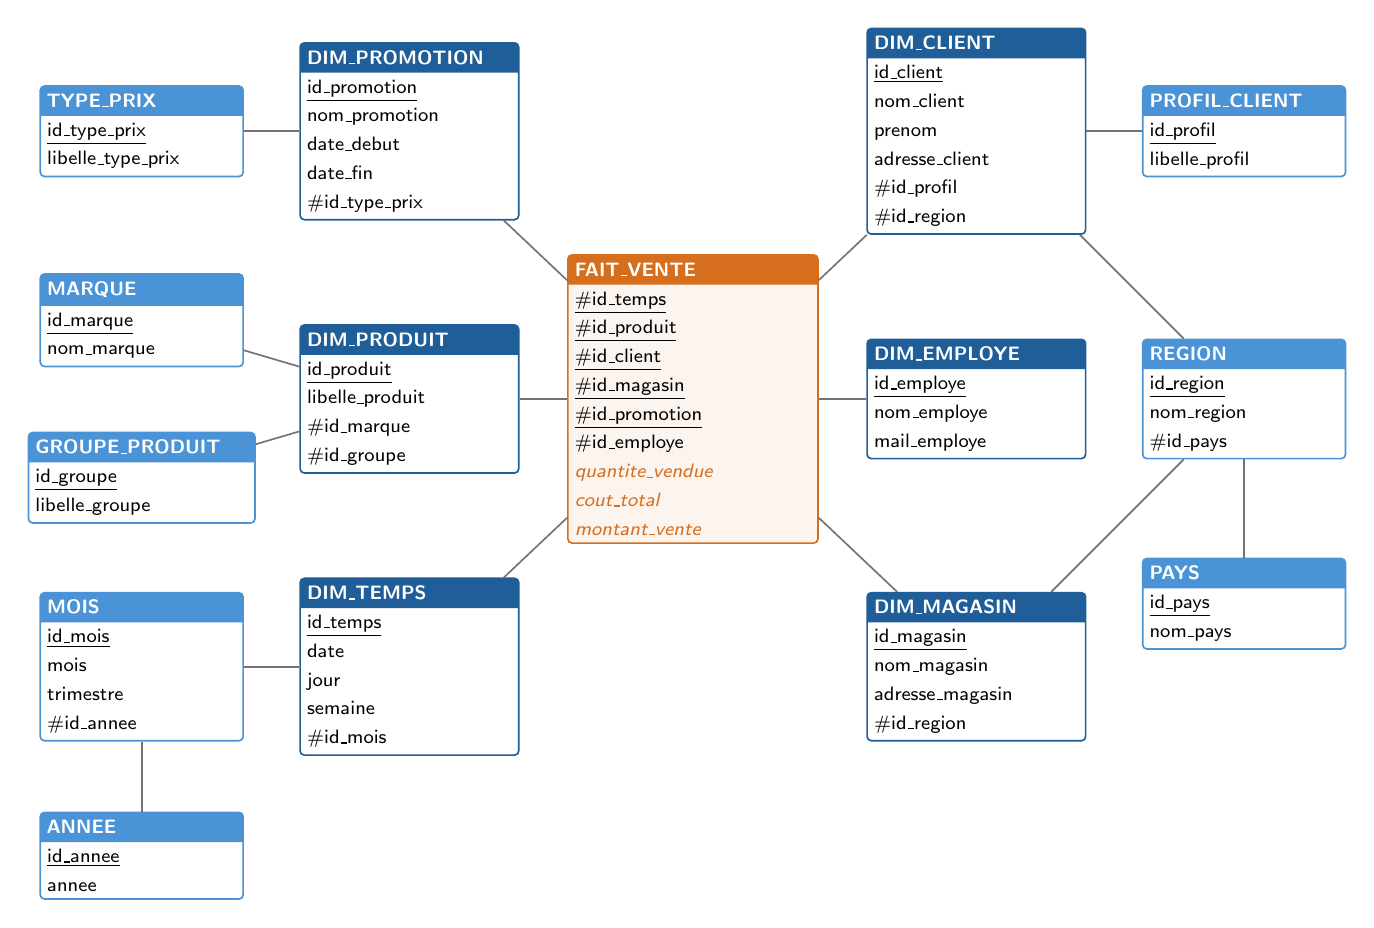
\begin{tikzpicture}
	\node[fait] (F) at (0,0) {\tb{FAIT\_VENTE}{\pk{\fk{id\_temps}}\\ \pk{\fk{id\_produit}}\\ \pk{\fk{id\_client}}\\ \pk{\fk{id\_magasin}}\\ \pk{\fk{id\_promotion}}\\ \fk{id\_employe}\\ \mes{quantite\_vendue}\\ \mes{cout\_total}\\ \mes{montant\_vente}}};

	% Gauche : dimensions de 1er niveau
	\node[tbl] (PR) at (-3.6, 3.4) {\tb{DIM\_PROMOTION}{\pk{id\_promotion}\\ nom\_promotion\\ date\_debut\\ date\_fin\\ \fk{id\_type\_prix}}};
	\node[tbl] (P)  at (-3.6, 0)   {\tb{DIM\_PRODUIT}{\pk{id\_produit}\\ libelle\_produit\\ \fk{id\_marque}\\ \fk{id\_groupe}}};
	\node[tbl] (T)  at (-3.6,-3.4) {\tb{DIM\_TEMPS}{\pk{id\_temps}\\ date\\ jour\\ semaine\\ \fk{id\_mois}}};
	% Gauche : sous-tables
	\node[sous] (TP) at (-7, 3.4)  {\tb{TYPE\_PRIX}{\pk{id\_type\_prix}\\ libelle\_type\_prix}};
	\node[sous] (MA) at (-7, 1.0)  {\tb{MARQUE}{\pk{id\_marque}\\ nom\_marque}};
	\node[sous=2.7cm] (G)  at (-7,-1.0)  {\tb{GROUPE\_PRODUIT}{\pk{id\_groupe}\\ libelle\_groupe}};
	\node[sous] (MO) at (-7,-3.4)  {\tb{MOIS}{\pk{id\_mois}\\ mois\\ trimestre\\ \fk{id\_annee}}};
	\node[sous] (AN) at (-7,-5.8)  {\tb{ANNEE}{\pk{id\_annee}\\ annee}};

	% Droite : dimensions de 1er niveau
	\node[tbl] (C) at (3.6, 3.4) {\tb{DIM\_CLIENT}{\pk{id\_client}\\ nom\_client\\ prenom\\ adresse\_client\\ \fk{id\_profil}\\ \fk{id\_region}}};
	\node[tbl] (E) at (3.6, 0)   {\tb{DIM\_EMPLOYE}{\pk{id\_employe}\\ nom\_employe\\ mail\_employe}};
	\node[tbl] (M) at (3.6,-3.4) {\tb{DIM\_MAGASIN}{\pk{id\_magasin}\\ nom\_magasin\\ adresse\_magasin\\ \fk{id\_region}}};
	% Droite : sous-tables
	\node[sous] (PC) at (7, 3.4)  {\tb{PROFIL\_CLIENT}{\pk{id\_profil}\\ libelle\_profil}};
	\node[sous] (RE) at (7, 0)    {\tb{REGION}{\pk{id\_region}\\ nom\_region\\ \fk{id\_pays}}};
	\node[sous] (PA) at (7,-2.6)  {\tb{PAYS}{\pk{id\_pays}\\ nom\_pays}};

	\foreach \d in {PR, P, T, C, E, M} \draw[lien] (F) -- (\d);
	\draw[lien] (PR) -- (TP);
	\draw[lien] (P) -- (MA);  \draw[lien] (P) -- (G);
	\draw[lien] (T) -- (MO);  \draw[lien] (MO) -- (AN);
	\draw[lien] (C) -- (PC);
	\draw[lien] (C) -- (RE);  \draw[lien] (M) -- (RE);
	\draw[lien] (RE) -- (PA);
\end{tikzpicture}
\end{adjustbox}
\legende
\end{center}

% ---------------------------------------------------------------------
\newpage
\subsection*{3. Avantages et inconvénients}
\phantomsection
\addcontentsline{toc}{subsection}{3. Avantages et inconvénients}

\begin{center}
\small
\begin{tabularx}{\linewidth}{>{\bfseries}l X X}
	\toprule
	& \textbf{Modèle en étoile} & \textbf{Modèle en flocon} \\
	\midrule
	Structure & Une table par dimension, dénormalisée & Dimensions normalisées en sous-tables \\
	Requêtes & \good{} Simples, peu de jointures (fait $\leftrightarrow$ dimension) & \bad{} Plus de jointures, requêtes plus longues à écrire \\
	Performances & \good{} Rapides en lecture, adaptées à l'OLAP & \bad{} Plus lentes sur de gros volumes \\
	Stockage & \bad{} Redondance (ex.~: le pays répété pour chaque client) & \good{} Pas de redondance, moins d'espace disque \\
	Mise à jour & \bad{} Une modification se répète sur de nombreuses lignes & \good{} Une seule ligne à modifier, cohérence garantie \\
	Hiérarchies & \bad{} Implicites, dans les colonnes & \good{} Explicites, faciles à parcourir (\textit{drill-down}) \\
	Lisibilité & \good{} Simple à comprendre pour les métiers & \bad{} Schéma plus complexe \\
	Usage & Data marts, outils de reporting (Power BI\dots) & Dimensions volumineuses ou hiérarchies partagées \\
	\bottomrule
\end{tabularx}
\end{center}

\noindent En pratique, l'\textbf{étoile} est privilégiée pour la restitution (les dimensions sont petites face à la table de faits, donc la redondance coûte peu). Le \textbf{flocon} se justifie quand une dimension est très volumineuse ou qu'une hiérarchie est partagée (ici Région/Pays entre clients et magasins).

% =====================================================================
%  EXERCICE 3
% =====================================================================
\newpage
\section*{Exercice 3~: réservation d'hôtels}
\addcontentsline{toc}{section}{Exercice 3~: réservation d'hôtels}

% ---------------------------------------------------------------------
\subsection*{1. Règles de gestion}
\phantomsection
\addcontentsline{toc}{subsection}{1. Règles de gestion}

\begin{enumerate}[label=\textbf{RG\arabic*}~:, leftmargin=*]
	\item Un hôtel possède un \textbf{classement} de 1 à 5 étoiles.
	\item Un hôtel appartient à \textbf{0 ou 1 chaîne hôtelière}~; une chaîne regroupe un ou plusieurs hôtels.
	\item Un hôtel est situé à une adresse, dans une ville et un pays (Thierry voyage à l'étranger).
	\item Un hôtel est décrit par plusieurs \textbf{caractéristiques} (options~: piscine, spa, Wi-Fi\dots)~; une même caractéristique se retrouve dans plusieurs hôtels.
	\item Un hôtel possède plusieurs \textbf{chambres}~; une chambre appartient à un seul hôtel.
	\item Une chambre est d'un seul \textbf{type} (simple, double, suite\dots)~; un type concerne plusieurs chambres.
	\item Le \textbf{tarif journalier} dépend du \textbf{type de chambre} et de la \textbf{date de réservation} (saison, période).
	\item Un client effectue une ou plusieurs \textbf{réservations}~; une réservation est faite par un seul client.
	\item Une réservation porte sur une ou plusieurs chambres, pour une \textbf{période} définie par une date d'arrivée et une date de départ (départ postérieur à l'arrivée).
	\item Une chambre ne peut pas être réservée deux fois sur une même nuit~: elle n'est \textbf{disponible} que si aucune réservation ne couvre la période demandée.
	\item Le \textbf{montant} d'une réservation vaut le nombre de nuits multiplié par le tarif journalier appliqué (moins une éventuelle remise).
	\item Une réservation peut être \textbf{modifiée} (réduction de la période, comme Thierry) ou \textbf{annulée}.
\end{enumerate}

% ---------------------------------------------------------------------
\newpage
\subsection*{2. Modèle dimensionnel logique~: revenus de l'hôtel}
\phantomsection
\addcontentsline{toc}{subsection}{2. Modèle dimensionnel logique~: revenus de l'hôtel}

\begin{itemize}
	\item \textbf{Fait~:} la réservation (source du revenu). \textbf{Grain~:} une chambre réservée dans une réservation~; le numéro de réservation est une \textbf{dimension dégénérée}.
	\item \textbf{Mesures~:} \texttt{nb\_nuits}, \texttt{nb\_personnes}, \texttt{montant\_remise}, \texttt{montant\_total} (additives) et \texttt{tarif\_journalier} (non additive~: on en calcule la moyenne).
	\item La dimension Date joue \textbf{trois rôles}~: réservation (qui fixe le tarif, RG7), arrivée et départ. Les caractéristiques sont reliées aux hôtels par une \textbf{table pont} (n-n, RG4).
\end{itemize}

\begin{center}
\begin{adjustbox}{width=\linewidth}
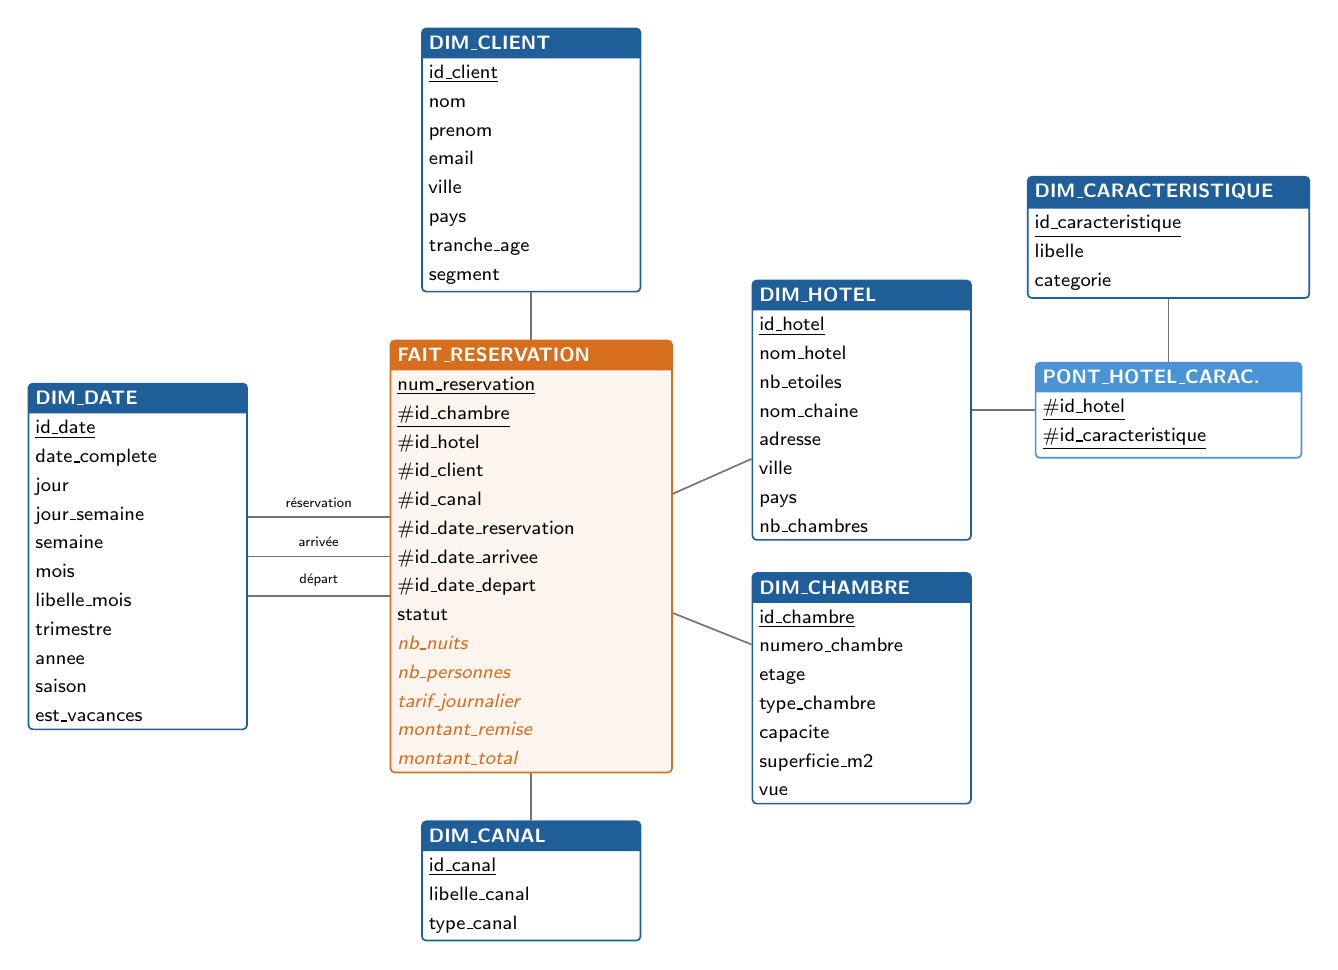
\begin{tikzpicture}
	\node[fait=3.4cm] (F) {\tb{FAIT\_RESERVATION}{\pk{num\_reservation}\\ \pk{\fk{id\_chambre}}\\ \fk{id\_hotel}\\ \fk{id\_client}\\ \fk{id\_canal}\\ \fk{id\_date\_reservation}\\ \fk{id\_date\_arrivee}\\ \fk{id\_date\_depart}\\ statut\\ \mes{nb\_nuits}\\ \mes{nb\_personnes}\\ \mes{tarif\_journalier}\\ \mes{montant\_remise}\\ \mes{montant\_total}}};

	\node[tbl, anchor=east] (D) at ($(F.west)+(-1.8,0)$) {\tb{DIM\_DATE}{\pk{id\_date}\\ date\_complete\\ jour\\ jour\_semaine\\ semaine\\ mois\\ libelle\_mois\\ trimestre\\ annee\\ saison\\ est\_vacances}};
	\node[tbl, anchor=south] (C) at ($(F.north)+(0,0.6)$) {\tb{DIM\_CLIENT}{\pk{id\_client}\\ nom\\ prenom\\ email\\ ville\\ pays\\ tranche\_age\\ segment}};
	\node[tbl, anchor=north] (CA) at ($(F.south)+(0,-0.6)$) {\tb{DIM\_CANAL}{\pk{id\_canal}\\ libelle\_canal\\ type\_canal}};
	\node[tbl, anchor=south west] (H) at ($(F.east)+(1,0.2)$) {\tb{DIM\_HOTEL}{\pk{id\_hotel}\\ nom\_hotel\\ nb\_etoiles\\ nom\_chaine\\ adresse\\ ville\\ pays\\ nb\_chambres}};
	\node[tbl, anchor=north west] (CH) at ($(F.east)+(1,-0.2)$) {\tb{DIM\_CHAMBRE}{\pk{id\_chambre}\\ numero\_chambre\\ etage\\ type\_chambre\\ capacite\\ superficie\_m2\\ vue}};
	\node[sous=3.2cm, anchor=west] (PO) at ($(H.east)+(0.8,0)$) {\tb{PONT\_HOTEL\_CARAC.}{\pk{\fk{id\_hotel}}\\ \pk{\fk{id\_caracteristique}}}};
	\node[tbl=3.4cm, anchor=south] (CR) at ($(PO.north)+(0,0.8)$) {\tb{DIM\_CARACTERISTIQUE}{\pk{id\_caracteristique}\\ libelle\\ categorie}};

	\draw[lien] ($(F.west)+(0,0.5)$)  -- node[above, font=\tiny]{réservation} ($(D.east)+(0,0.5)$);
	\draw[lien] ($(F.west)+(0,0)$)    -- node[above, font=\tiny]{arrivée}     ($(D.east)+(0,0)$);
	\draw[lien] ($(F.west)+(0,-0.5)$) -- node[above, font=\tiny]{départ}      ($(D.east)+(0,-0.5)$);
	\foreach \d in {C, CA, H, CH} \draw[lien] (F) -- (\d);
	\draw[lien] (H) -- (PO);
	\draw[lien] (PO) -- (CR);
\end{tikzpicture}
\end{adjustbox}
\legende
\end{center}

% ---------------------------------------------------------------------
\newpage
\noindent \textbf{MLD (notation relationnelle)~:}

\begin{tcolorbox}[colback=white, colframe=title1]
\small
\textbf{DIM\_DATE} (\pk{id\_date}, date\_complete, jour, jour\_semaine, semaine, mois, libelle\_mois, trimestre, annee, saison, est\_vacances) \\
\textbf{DIM\_CLIENT} (\pk{id\_client}, nom, prenom, email, ville, pays, tranche\_age, segment) \\
\textbf{DIM\_HOTEL} (\pk{id\_hotel}, nom\_hotel, nb\_etoiles, nom\_chaine, adresse, ville, pays, nb\_chambres) \\
\textbf{DIM\_CHAMBRE} (\pk{id\_chambre}, numero\_chambre, etage, type\_chambre, capacite, superficie\_m2, vue) \\
\textbf{DIM\_CANAL} (\pk{id\_canal}, libelle\_canal, type\_canal) \\
\textbf{DIM\_CARACTERISTIQUE} (\pk{id\_caracteristique}, libelle, categorie) \\
\textbf{PONT\_HOTEL\_CARACTERISTIQUE} (\pk{\fk{id\_hotel}, \fk{id\_caracteristique}}) \\
\textbf{FAIT\_RESERVATION} (\pk{num\_reservation, \fk{id\_chambre}}, \fk{id\_hotel}, \fk{id\_client}, \fk{id\_canal}, \fk{id\_date\_reservation}, \fk{id\_date\_arrivee}, \fk{id\_date\_depart}, statut, nb\_nuits, nb\_personnes, tarif\_journalier, montant\_remise, montant\_total)
\end{tcolorbox}

\noindent Ce modèle répond aux questions d'analyse des revenus~: chiffre d'affaires par chaîne, hôtel, nombre d'étoiles ou type de chambre~; évolution selon la saison ou le mois d'arrivée~; tarif moyen par type de chambre~; durée moyenne de séjour~; part des réservations modifiées ou annulées~; revenu selon le canal ou le pays d'origine du client.

% =====================================================================
%  EXERCICE 4
% =====================================================================
\newpage
\section*{Exercice 4~: modèle physique de données}
\addcontentsline{toc}{section}{Exercice 4~: modèle physique de données}

\noindent Le modèle physique traduit le MLD de l'exercice 3 pour un SGBD précis, ici \textbf{PostgreSQL}~: chaque attribut reçoit un \textbf{type} de données, et on précise les \textbf{contraintes} (clés, valeurs autorisées, \texttt{NOT NULL}). Le schéma est présenté page suivante.

\subsection*{Choix d'implémentation}
\phantomsection
\addcontentsline{toc}{subsection}{Choix d'implémentation}

\begin{center}
\small
\begin{tabularx}{\linewidth}{l X}
	\toprule
	\textbf{Élément} & \textbf{Choix} \\
	\midrule
	Clés des dimensions & \texttt{INTEGER}~: clés de substitution (\textit{surrogate keys}) attribuées par l'ETL, indépendantes des identifiants sources \\
	Clé de la date & \texttt{INTEGER} au format \texttt{AAAAMMJJ} (ex.~: \texttt{20270702})~: lisible et ordonnée \\
	Montants & \texttt{NUMERIC(p,2)}~: valeurs exactes, sans erreur d'arrondi (pas de \texttt{FLOAT}) \\
	Petits entiers & \texttt{SMALLINT} (étoiles, nuits, capacité, mois\dots) \\
	Textes & \texttt{VARCHAR(n)} dimensionnés selon la donnée \\
	Booléens & \texttt{BOOLEAN} (\texttt{est\_vacances}) \\
	\bottomrule
\end{tabularx}
\end{center}

\subsection*{Contraintes}
\phantomsection
\addcontentsline{toc}{subsection}{Contraintes}

\begin{itemize}
	\item \textbf{Intégrité~:} \texttt{PRIMARY KEY} sur chaque table, \texttt{FOREIGN KEY} du fait vers les dimensions, \texttt{NOT NULL} sur les attributs obligatoires (\texttt{nom\_chaine} reste \texttt{NULL} pour un hôtel indépendant).
	\item \textbf{Domaines (\texttt{CHECK})~:} \texttt{nb\_etoiles} entre 1 et 5~; \texttt{statut} $\in$ \{Confirmée, Modifiée, Annulée\}~; \texttt{type\_chambre} $\in$ \{Simple, Double, Twin, Suite, Familiale\}~; \texttt{nb\_nuits}, \texttt{nb\_personnes} $> 0$~; montants $\geq 0$.
	\item \textbf{Cohérence des dates~:} date de réservation $\leq$ date d'arrivée $<$ date de départ.
	\item \textbf{Performances~:} index sur les clés étrangères de \texttt{FAIT\_RESERVATION}, utilisées dans toutes les jointures.
\end{itemize}

\noindent Le script SQL correspondant (\texttt{sql/ex4\_hotel\_datamart.sql}) a été testé avec un jeu d'essai (\texttt{sql/ex4\_jeu\_essai.sql})~: les contraintes rejettent bien un départ antérieur à l'arrivée, une chambre inexistante ou un hôtel à 6 étoiles.

% ---------------------------------------------------------------------
\begin{landscape}
\subsection*{Schéma du modèle physique}
\phantomsection
\addcontentsline{toc}{subsection}{Schéma du modèle physique}

\begin{center}
\begin{adjustbox}{max width=\linewidth, max totalheight=0.78\textheight}
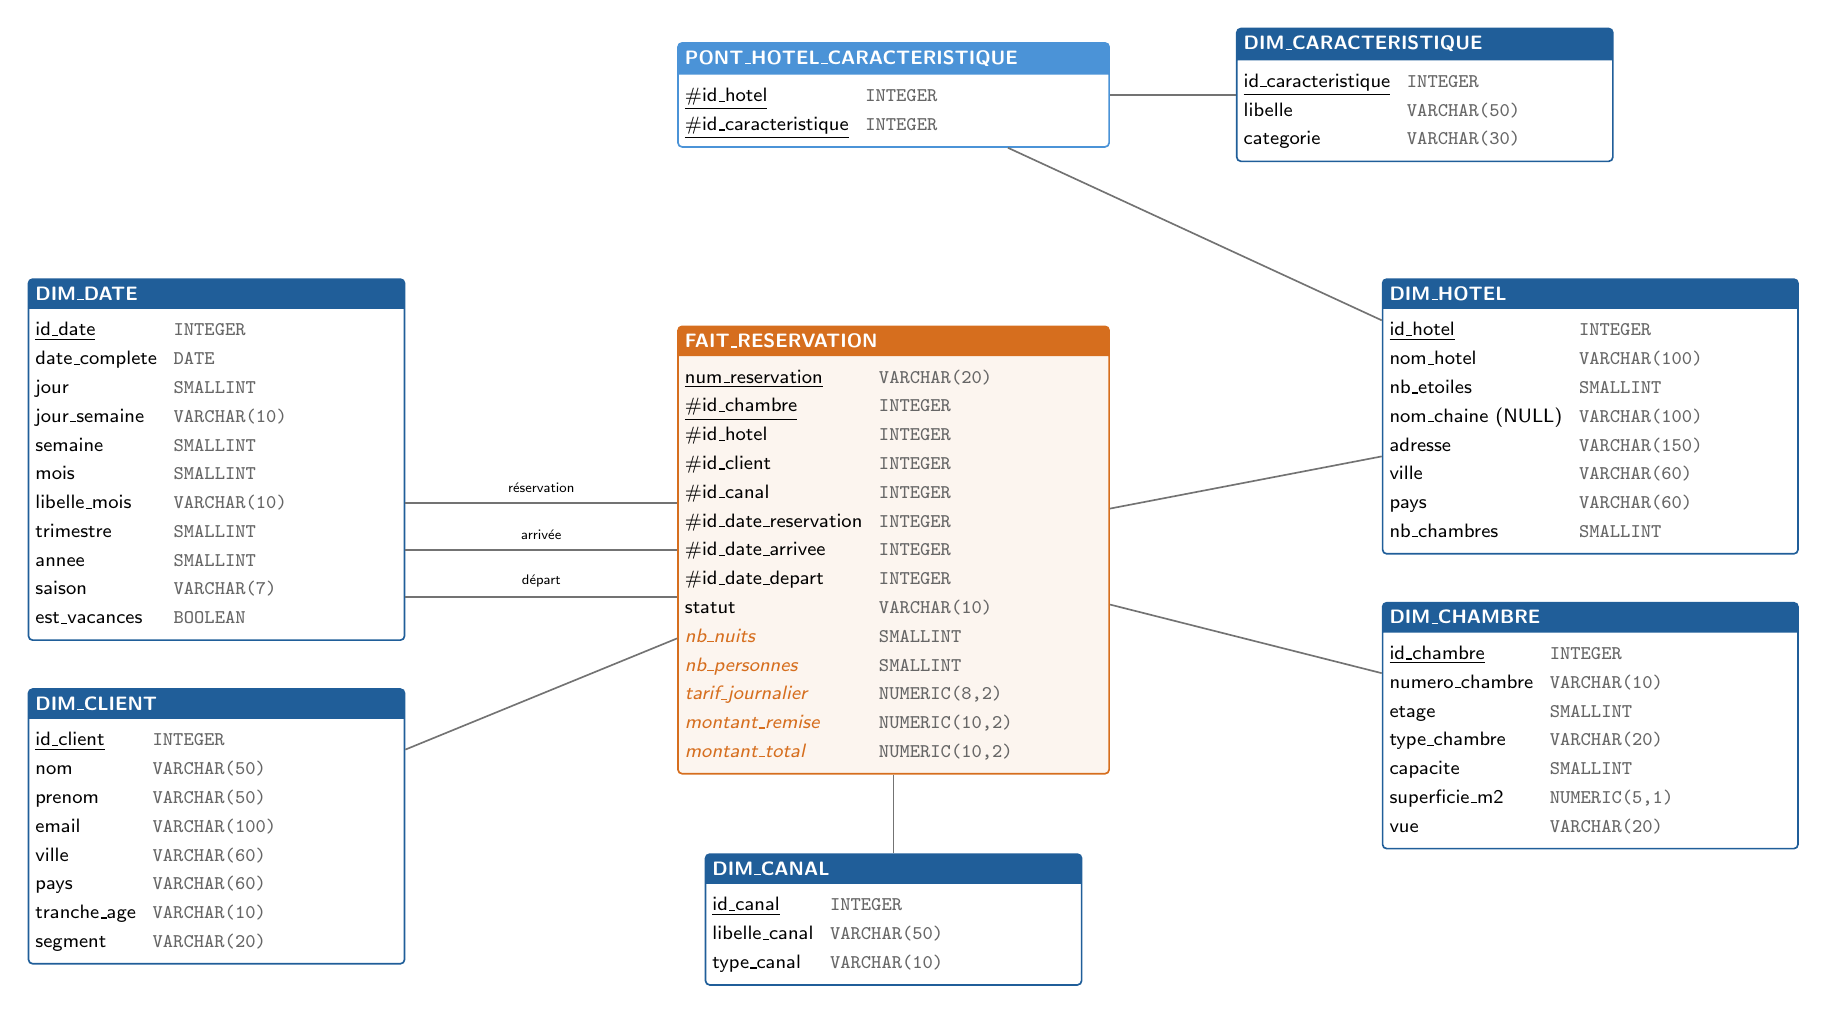
\begin{tikzpicture}
	\node[fait=5.3cm, anchor=north] (F) at (0,0) {\tb{FAIT\_RESERVATION}{\begin{phys}
		\pk{num\_reservation} & VARCHAR(20) \\
		\pk{\fk{id\_chambre}} & INTEGER \\
		\fk{id\_hotel} & INTEGER \\
		\fk{id\_client} & INTEGER \\
		\fk{id\_canal} & INTEGER \\
		\fk{id\_date\_reservation} & INTEGER \\
		\fk{id\_date\_arrivee} & INTEGER \\
		\fk{id\_date\_depart} & INTEGER \\
		statut & VARCHAR(10) \\
		\mes{nb\_nuits} & SMALLINT \\
		\mes{nb\_personnes} & SMALLINT \\
		\mes{tarif\_journalier} & NUMERIC(8,2) \\
		\mes{montant\_remise} & NUMERIC(10,2) \\
		\mes{montant\_total} & NUMERIC(10,2) \\
	\end{phys}}};

	\node[tbl=4.6cm, anchor=north east] (D) at (-6.2,0.6) {\tb{DIM\_DATE}{\begin{phys}
		\pk{id\_date} & INTEGER \\
		date\_complete & DATE \\
		jour & SMALLINT \\
		jour\_semaine & VARCHAR(10) \\
		semaine & SMALLINT \\
		mois & SMALLINT \\
		libelle\_mois & VARCHAR(10) \\
		trimestre & SMALLINT \\
		annee & SMALLINT \\
		saison & VARCHAR(7) \\
		est\_vacances & BOOLEAN \\
	\end{phys}}};
	\node[tbl=4.6cm, anchor=north east] (C) at ($(D.south east)+(0,-0.6)$) {\tb{DIM\_CLIENT}{\begin{phys}
		\pk{id\_client} & INTEGER \\
		nom & VARCHAR(50) \\
		prenom & VARCHAR(50) \\
		email & VARCHAR(100) \\
		ville & VARCHAR(60) \\
		pays & VARCHAR(60) \\
		tranche\_age & VARCHAR(10) \\
		segment & VARCHAR(20) \\
	\end{phys}}};

	\node[tbl=4.6cm, anchor=north] (CA) at ($(F.south)+(0,-1)$) {\tb{DIM\_CANAL}{\begin{phys}
		\pk{id\_canal} & INTEGER \\
		libelle\_canal & VARCHAR(50) \\
		type\_canal & VARCHAR(10) \\
	\end{phys}}};

	\node[tbl=5.1cm, anchor=north west] (H) at (6.2,0.6) {\tb{DIM\_HOTEL}{\begin{phys}
		\pk{id\_hotel} & INTEGER \\
		nom\_hotel & VARCHAR(100) \\
		nb\_etoiles & SMALLINT \\
		nom\_chaine (NULL) & VARCHAR(100) \\
		adresse & VARCHAR(150) \\
		ville & VARCHAR(60) \\
		pays & VARCHAR(60) \\
		nb\_chambres & SMALLINT \\
	\end{phys}}};
	\node[tbl=5.1cm, anchor=north west] (CH) at ($(H.south west)+(0,-0.6)$) {\tb{DIM\_CHAMBRE}{\begin{phys}
		\pk{id\_chambre} & INTEGER \\
		numero\_chambre & VARCHAR(10) \\
		etage & SMALLINT \\
		type\_chambre & VARCHAR(20) \\
		capacite & SMALLINT \\
		superficie\_m2 & NUMERIC(5,1) \\
		vue & VARCHAR(20) \\
	\end{phys}}};

	\node[sous=5.3cm, anchor=north] (PO) at ($(F.north)+(0,3.6)$) {\tb{PONT\_HOTEL\_CARACTERISTIQUE}{\begin{phys}
		\pk{\fk{id\_hotel}} & INTEGER \\
		\pk{\fk{id\_caracteristique}} & INTEGER \\
	\end{phys}}};
	\node[tbl=4.6cm, anchor=west] (CR) at ($(PO.east)+(1.6,0)$) {\tb{DIM\_CARACTERISTIQUE}{\begin{phys}
		\pk{id\_caracteristique} & INTEGER \\
		libelle & VARCHAR(50) \\
		categorie & VARCHAR(30) \\
	\end{phys}}};

	\foreach \dy/\role in {0.6/réservation, 0/arrivée, -0.6/départ}
		\draw[lien] ($(F.west)+(0,\dy)$) -- node[above, font=\tiny]{\role} ({$(F.west)+(0,\dy)$} -| D.east);
	\draw[lien] (F) -- (C);
	\draw[lien] (F) -- (CA);
	\draw[lien] (F) -- (H);
	\draw[lien] (F) -- (CH);
	\draw[lien] (PO) -- (H);
	\draw[lien] (PO) -- (CR);
\end{tikzpicture}
\end{adjustbox}
\legende
\end{center}
\end{landscape}

% =====================================================================
%  EXERCICE 5
% =====================================================================
\newpage
\section*{Exercice 5~: data mart des ventes de meubles}
\addcontentsline{toc}{section}{Exercice 5~: data mart des ventes de meubles}

\begin{itemize}
	\item \textbf{Fait à observer~:} la vente.
	\item \textbf{Axes d'analyse~:} le lieu de distribution (enseigne, surface, adresse, département, région), le temps (mois, semestre, année) et le type de vente.
	\item \textbf{Mesures~:} le \textbf{nombre d'articles} vendus et le \textbf{chiffre d'affaires}.
	\item \textbf{Grain~:} les ventes d'un type donné, dans un lieu de distribution, sur un mois.
\end{itemize}

% ---------------------------------------------------------------------
\subsection*{a) Modèle en étoile}
\phantomsection
\addcontentsline{toc}{subsection}{a) Modèle en étoile}

\vspace{0.5cm}
\begin{center}
\begin{adjustbox}{width=0.9\linewidth}
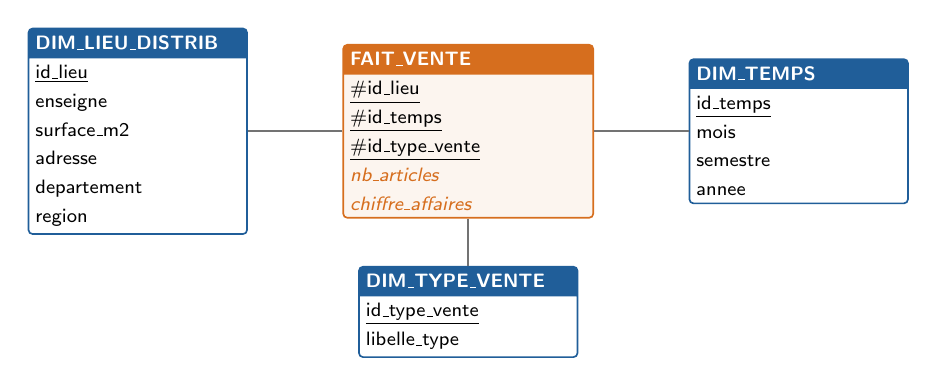
\begin{tikzpicture}
	\node[fait] (F) {\tb{FAIT\_VENTE}{\pk{\fk{id\_lieu}}\\ \pk{\fk{id\_temps}}\\ \pk{\fk{id\_type\_vente}}\\ \mes{nb\_articles}\\ \mes{chiffre\_affaires}}};
	\node[tbl, anchor=east] (L) at ($(F.west)+(-1.2,0)$) {\tb{DIM\_LIEU\_DISTRIB}{\pk{id\_lieu}\\ enseigne\\ surface\_m2\\ adresse\\ departement\\ region}};
	\node[tbl, anchor=west] (T) at ($(F.east)+(1.2,0)$) {\tb{DIM\_TEMPS}{\pk{id\_temps}\\ mois\\ semestre\\ annee}};
	\node[tbl, anchor=north] (TV) at ($(F.south)+(0,-0.6)$) {\tb{DIM\_TYPE\_VENTE}{\pk{id\_type\_vente}\\ libelle\_type}};
	\foreach \d in {L, T, TV} \draw[lien] (F) -- (\d);
\end{tikzpicture}
\end{adjustbox}
\legende
\end{center}

% ---------------------------------------------------------------------
\newpage
\subsection*{b) Modèle en flocon}
\phantomsection
\addcontentsline{toc}{subsection}{b) Modèle en flocon}

\noindent On normalise les hiérarchies~: Lieu $\rightarrow$ Enseigne, Lieu $\rightarrow$ Département $\rightarrow$ Région, et Mois $\rightarrow$ Semestre $\rightarrow$ Année.

\vspace{0.5cm}
\begin{center}
\begin{adjustbox}{width=0.85\linewidth}
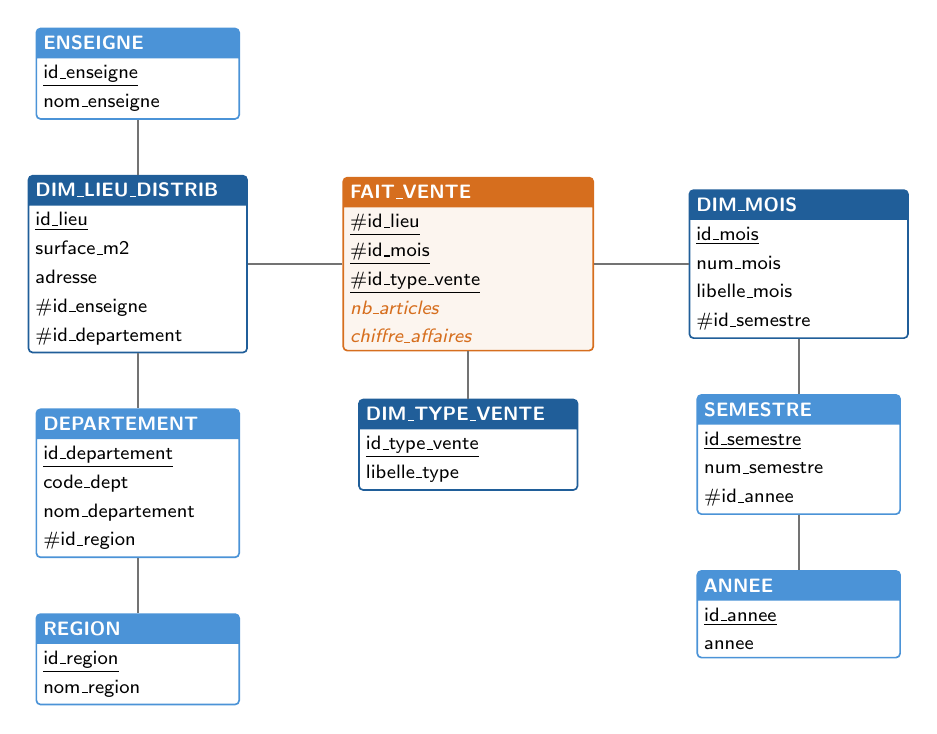
\begin{tikzpicture}
	\node[fait] (F) {\tb{FAIT\_VENTE}{\pk{\fk{id\_lieu}}\\ \pk{\fk{id\_mois}}\\ \pk{\fk{id\_type\_vente}}\\ \mes{nb\_articles}\\ \mes{chiffre\_affaires}}};
	\node[tbl, anchor=east] (L) at ($(F.west)+(-1.2,0)$) {\tb{DIM\_LIEU\_DISTRIB}{\pk{id\_lieu}\\ surface\_m2\\ adresse\\ \fk{id\_enseigne}\\ \fk{id\_departement}}};
	\node[sous, anchor=south] (EN) at ($(L.north)+(0,0.7)$) {\tb{ENSEIGNE}{\pk{id\_enseigne}\\ nom\_enseigne}};
	\node[sous, anchor=north] (DE) at ($(L.south)+(0,-0.7)$) {\tb{DEPARTEMENT}{\pk{id\_departement}\\ code\_dept\\ nom\_departement\\ \fk{id\_region}}};
	\node[sous, anchor=north] (RE) at ($(DE.south)+(0,-0.7)$) {\tb{REGION}{\pk{id\_region}\\ nom\_region}};

	\node[tbl, anchor=west] (MO) at ($(F.east)+(1.2,0)$) {\tb{DIM\_MOIS}{\pk{id\_mois}\\ num\_mois\\ libelle\_mois\\ \fk{id\_semestre}}};
	\node[sous, anchor=north] (SE) at ($(MO.south)+(0,-0.7)$) {\tb{SEMESTRE}{\pk{id\_semestre}\\ num\_semestre\\ \fk{id\_annee}}};
	\node[sous, anchor=north] (AN) at ($(SE.south)+(0,-0.7)$) {\tb{ANNEE}{\pk{id\_annee}\\ annee}};

	\node[tbl, anchor=north] (TV) at ($(F.south)+(0,-0.6)$) {\tb{DIM\_TYPE\_VENTE}{\pk{id\_type\_vente}\\ libelle\_type}};

	\foreach \d in {L, MO, TV} \draw[lien] (F) -- (\d);
	\draw[lien] (L) -- (EN);  \draw[lien] (L) -- (DE);  \draw[lien] (DE) -- (RE);
	\draw[lien] (MO) -- (SE); \draw[lien] (SE) -- (AN);
\end{tikzpicture}
\end{adjustbox}
\legende
\end{center}

% =====================================================================
%  EXERCICE 6
% =====================================================================
\newpage
\section*{Exercice 6~: flocon, étoile et constellation}
\addcontentsline{toc}{section}{Exercice 6~: flocon, étoile et constellation}

% ---------------------------------------------------------------------
\subsection*{a) Modèle en flocon}
\phantomsection
\addcontentsline{toc}{subsection}{a) Modèle en flocon}

\begin{itemize}
	\item \textbf{Fait~:} la vente~; \textbf{grain~:} un produit, dans un magasin, un jour donné.
	\item \textbf{Mesures~:} \texttt{quantite\_vendue} et \texttt{benefice}.
	\item \textbf{Temps~:} deux hiérarchies parallèles, Jour $\rightarrow$ Semaine $\rightarrow$ Année et Jour $\rightarrow$ Mois $\rightarrow$ Année. Une semaine peut chevaucher deux mois~: la semaine n'est donc pas un niveau du mois, les deux branches se rejoignent seulement au niveau Année.
	\item \textbf{Localisation~:} Magasin $\rightarrow$ Ville $\rightarrow$ Pays.
\end{itemize}

\vspace{0.3cm}
\begin{center}
\begin{adjustbox}{width=\linewidth}
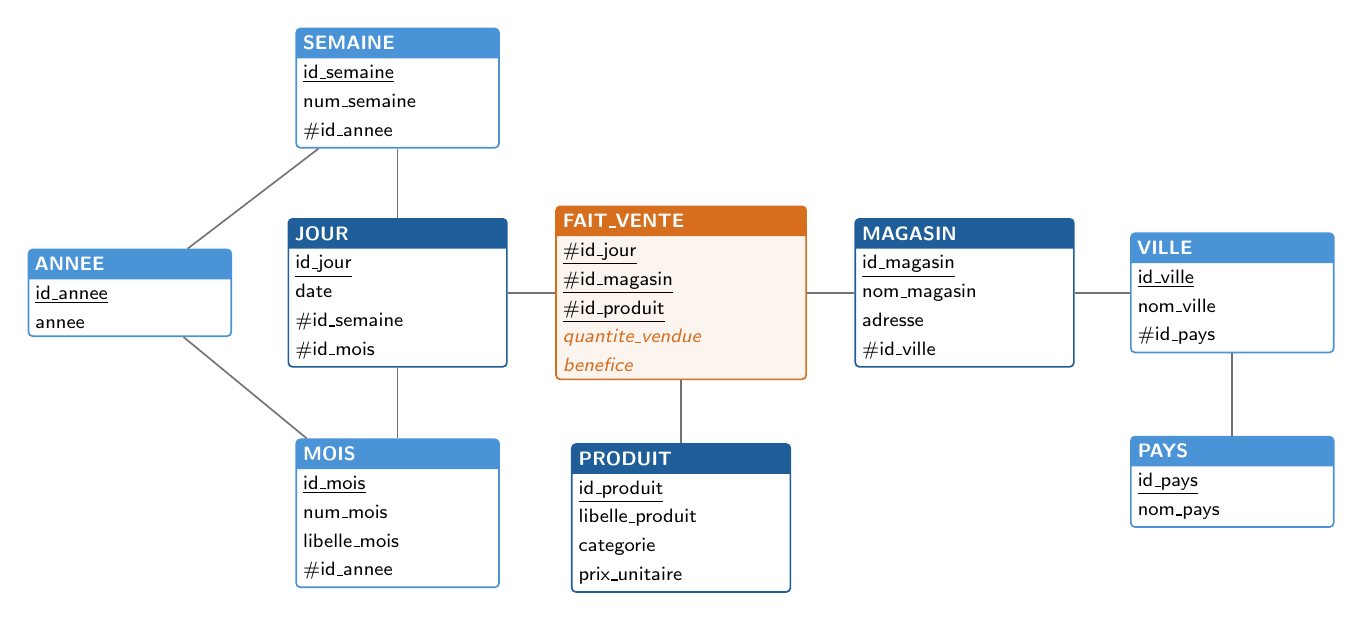
\begin{tikzpicture}
	\node[fait] (F) at (0,0) {\tb{FAIT\_VENTE}{\pk{\fk{id\_jour}}\\ \pk{\fk{id\_magasin}}\\ \pk{\fk{id\_produit}}\\ \mes{quantite\_vendue}\\ \mes{benefice}}};

	\node[tbl] (J)  at (-3.6, 0)   {\tb{JOUR}{\pk{id\_jour}\\ date\\ \fk{id\_semaine}\\ \fk{id\_mois}}};
	\node[sous] (S) at (-3.6, 2.6) {\tb{SEMAINE}{\pk{id\_semaine}\\ num\_semaine\\ \fk{id\_annee}}};
	\node[sous] (M) at (-3.6,-2.8) {\tb{MOIS}{\pk{id\_mois}\\ num\_mois\\ libelle\_mois\\ \fk{id\_annee}}};
	\node[sous] (A) at (-7, 0)     {\tb{ANNEE}{\pk{id\_annee}\\ annee}};

	\node[tbl] (MG) at (3.6, 0)    {\tb{MAGASIN}{\pk{id\_magasin}\\ nom\_magasin\\ adresse\\ \fk{id\_ville}}};
	\node[sous] (V) at (7, 0)      {\tb{VILLE}{\pk{id\_ville}\\ nom\_ville\\ \fk{id\_pays}}};
	\node[sous] (PA) at (7,-2.4)   {\tb{PAYS}{\pk{id\_pays}\\ nom\_pays}};

	\node[tbl, anchor=north] (P) at ($(F.south)+(0,-0.8)$) {\tb{PRODUIT}{\pk{id\_produit}\\ libelle\_produit\\ categorie\\ prix\_unitaire}};

	\foreach \d in {J, MG, P} \draw[lien] (F) -- (\d);
	\draw[lien] (J) -- (S); \draw[lien] (J) -- (M);
	\draw[lien] (S) -- (A); \draw[lien] (M) -- (A);
	\draw[lien] (MG) -- (V); \draw[lien] (V) -- (PA);
\end{tikzpicture}
\end{adjustbox}
\legende
\end{center}

% ---------------------------------------------------------------------
\newpage
\subsection*{b) Modèle en étoile}
\phantomsection
\addcontentsline{toc}{subsection}{b) Modèle en étoile}

\noindent On \textbf{réduit les hiérarchies} en fusionnant leurs niveaux dans une seule table de dimension~: Jour, Semaine, Mois et Année deviennent la dimension \texttt{DIM\_TEMPS}~; Magasin, Ville et Pays deviennent \texttt{DIM\_MAGASIN}. La table de faits reste identique.

\vspace{0.5cm}
\begin{center}
\begin{adjustbox}{width=0.9\linewidth}
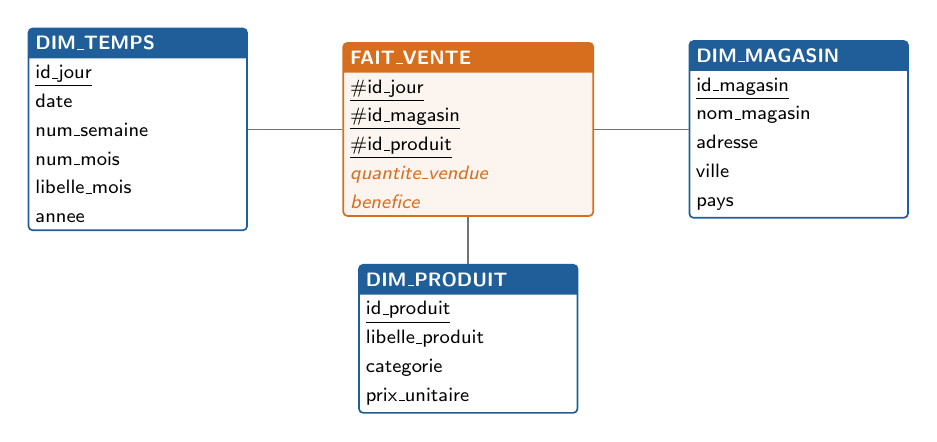
\begin{tikzpicture}
	\node[fait] (F) {\tb{FAIT\_VENTE}{\pk{\fk{id\_jour}}\\ \pk{\fk{id\_magasin}}\\ \pk{\fk{id\_produit}}\\ \mes{quantite\_vendue}\\ \mes{benefice}}};
	\node[tbl, anchor=east] (T) at ($(F.west)+(-1.2,0)$) {\tb{DIM\_TEMPS}{\pk{id\_jour}\\ date\\ num\_semaine\\ num\_mois\\ libelle\_mois\\ annee}};
	\node[tbl, anchor=west] (M) at ($(F.east)+(1.2,0)$) {\tb{DIM\_MAGASIN}{\pk{id\_magasin}\\ nom\_magasin\\ adresse\\ ville\\ pays}};
	\node[tbl, anchor=north] (P) at ($(F.south)+(0,-0.6)$) {\tb{DIM\_PRODUIT}{\pk{id\_produit}\\ libelle\_produit\\ categorie\\ prix\_unitaire}};
	\foreach \d in {T, M, P} \draw[lien] (F) -- (\d);
\end{tikzpicture}
\end{adjustbox}
\legende
\end{center}

% ---------------------------------------------------------------------
\newpage
\subsection*{c) Modèle en constellation}
\phantomsection
\addcontentsline{toc}{subsection}{c) Modèle en constellation}

\noindent Le nombre de commandes se mesure \textbf{par jour et par magasin}, sans le produit~: son grain est différent de celui de \texttt{FAIT\_VENTE}. On ajoute donc une seconde table de faits, \texttt{VENTE\_JOUR}, qui \textbf{partage} les dimensions Jour et Magasin (et leurs sous-tables) du flocon. Ces dimensions communes sont dites \textbf{conformes}~: elles permettent de croiser les deux faits (ex.~: quantité vendue moyenne par commande).

\vspace{0.5cm}
\begin{center}
\begin{adjustbox}{width=\linewidth}
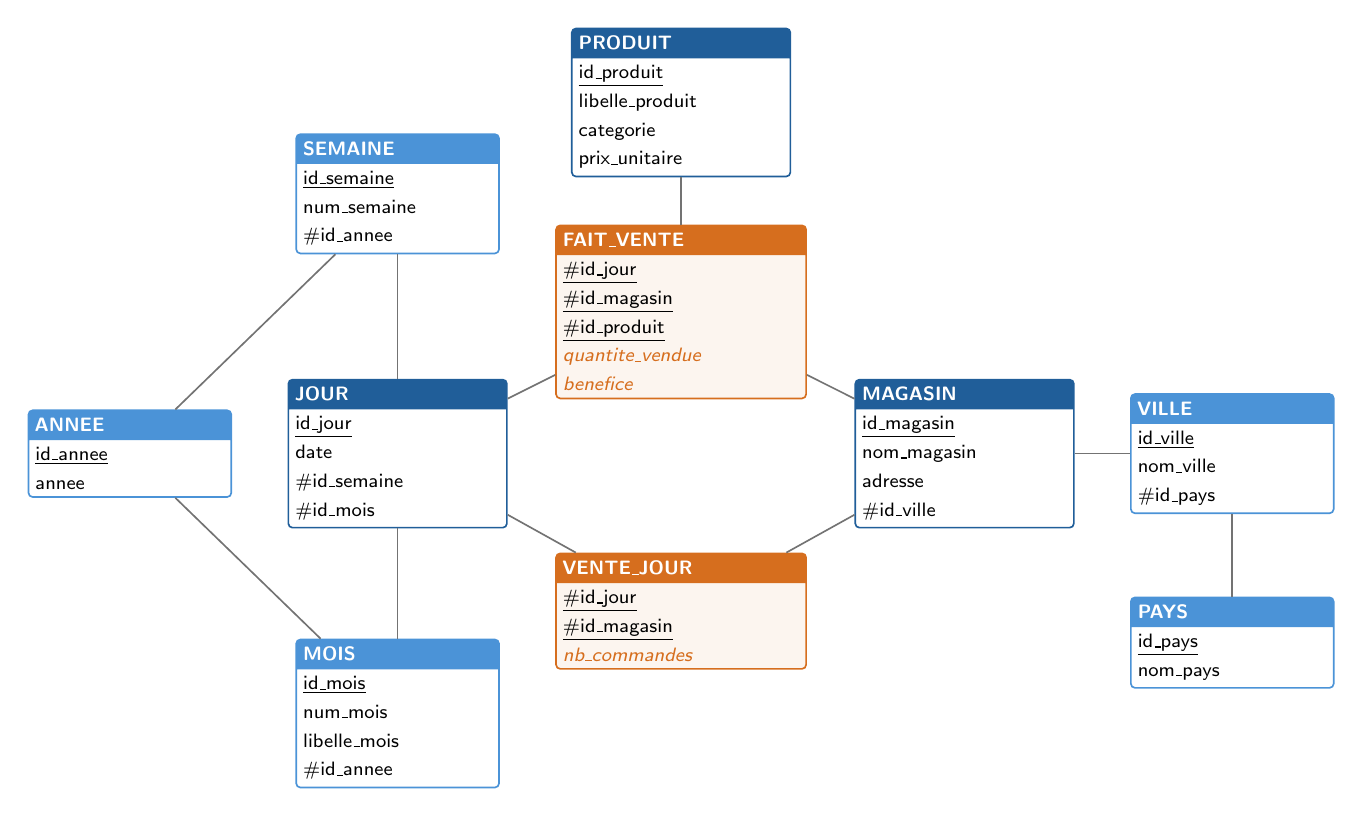
\begin{tikzpicture}
	\node[fait] (F)  at (0, 1.4)  {\tb{FAIT\_VENTE}{\pk{\fk{id\_jour}}\\ \pk{\fk{id\_magasin}}\\ \pk{\fk{id\_produit}}\\ \mes{quantite\_vendue}\\ \mes{benefice}}};
	\node[fait] (VJ) at (0,-2.4)  {\tb{VENTE\_JOUR}{\pk{\fk{id\_jour}}\\ \pk{\fk{id\_magasin}}\\ \mes{nb\_commandes}}};

	\node[tbl] (J)  at (-3.6,-0.4) {\tb{JOUR}{\pk{id\_jour}\\ date\\ \fk{id\_semaine}\\ \fk{id\_mois}}};
	\node[sous] (S) at (-3.6, 2.9) {\tb{SEMAINE}{\pk{id\_semaine}\\ num\_semaine\\ \fk{id\_annee}}};
	\node[sous] (M) at (-3.6,-3.7) {\tb{MOIS}{\pk{id\_mois}\\ num\_mois\\ libelle\_mois\\ \fk{id\_annee}}};
	\node[sous] (A) at (-7,-0.4)   {\tb{ANNEE}{\pk{id\_annee}\\ annee}};

	\node[tbl] (MG) at (3.6,-0.4)  {\tb{MAGASIN}{\pk{id\_magasin}\\ nom\_magasin\\ adresse\\ \fk{id\_ville}}};
	\node[sous] (V) at (7,-0.4)    {\tb{VILLE}{\pk{id\_ville}\\ nom\_ville\\ \fk{id\_pays}}};
	\node[sous] (PA) at (7,-2.8)   {\tb{PAYS}{\pk{id\_pays}\\ nom\_pays}};

	\node[tbl, anchor=south] (P) at ($(F.north)+(0,0.6)$) {\tb{PRODUIT}{\pk{id\_produit}\\ libelle\_produit\\ categorie\\ prix\_unitaire}};

	\foreach \d in {J, MG, P} \draw[lien] (F) -- (\d);
	\foreach \d in {J, MG} \draw[lien] (VJ) -- (\d);
	\draw[lien] (J) -- (S); \draw[lien] (J) -- (M);
	\draw[lien] (S) -- (A); \draw[lien] (M) -- (A);
	\draw[lien] (MG) -- (V); \draw[lien] (V) -- (PA);
\end{tikzpicture}
\end{adjustbox}
\legende
\end{center}

% =====================================================================
%  CONCLUSION
% =====================================================================
\newpage
\section*{Conclusion}
\addcontentsline{toc}{section}{Conclusion}

\noindent Ce workshop a suivi la démarche complète de modélisation d'un entrepôt de données~:
\begin{enumerate}
	\item \textbf{MCD $\rightarrow$ MLD}~: les associations 1-n deviennent des clés étrangères, les associations n-n des tables d'association (historisées si besoin)~;
	\item \textbf{modélisation dimensionnelle}~: identifier le fait, fixer son grain, choisir des mesures additives et des axes d'analyse~;
	\item \textbf{étoile, flocon ou constellation}~: dénormaliser pour la performance et la simplicité, normaliser les hiérarchies pour limiter la redondance, partager des dimensions conformes entre plusieurs faits~;
	\item \textbf{modèle physique}~: typer les attributs, poser les contraintes d'intégrité et les index selon le SGBD cible.
\end{enumerate}

\noindent Ces modèles ont une finalité \textbf{analytique et décisionnelle}~: ils préparent le projet d'entrepôt de données hospitalier, où la même démarche s'applique (faits~: consultations, hospitalisations~; dimensions~: patient, établissement, diagnostic, temps).


\end{document}
